\documentclass{beamer}


\usepackage[french,english]{babel}

\usepackage[T1]{fontenc}

\usepackage[utf8]{inputenc}


\usetheme{Warsaw}
\title{Résultats de l'heuristique}

\author{Clément Legrand}
\date{7 Juin 2018}

\begin{document}

\section{Exécution de l'heuristique}

\begin{frame}[plain]
\titlepage
\end{frame}

\begin{frame}{Exécution}
Algorithme légèrement différent.
\begin{block}{Détail}
\begin{itemize}
\item Calcul SI avec CW, et amélioration avec LK;
\item Boucle de $5000$ itérations en exécutant successivement EC, CE, LK.
\item On repart de la dernière solution globale toutes les $25$ itérations sans améliorations;
\item Si on trouve une amélioration, on met à jour la solution globale;
\item Toutes les $100$ itérations sans améliorations, on change de fonction de pénalisation.
\item A la fin on essaie de supprimer toutes les routes qui n'ont qu'un client.
\end{itemize}
\end{block}
\end{frame}

\section{Présentation résultats}

\subsection{Résultats}

\begin{frame}{Instance A-n37-k06}
Exécution de l'heuristique sur des instances de la littérature:
\begin{center}
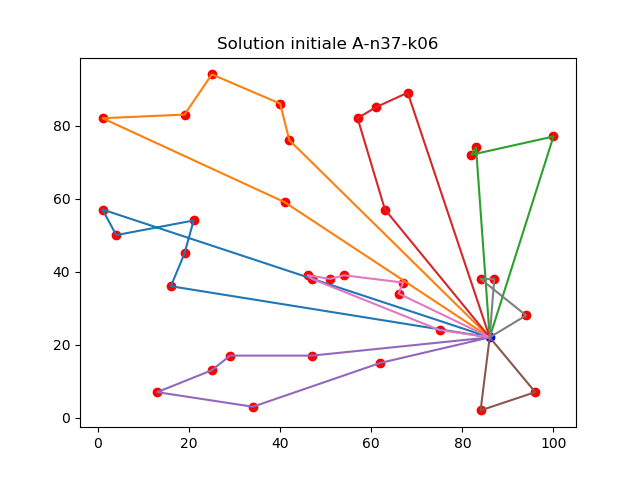
\includegraphics[scale=0.3]{initiale_A-n37-k06.png}
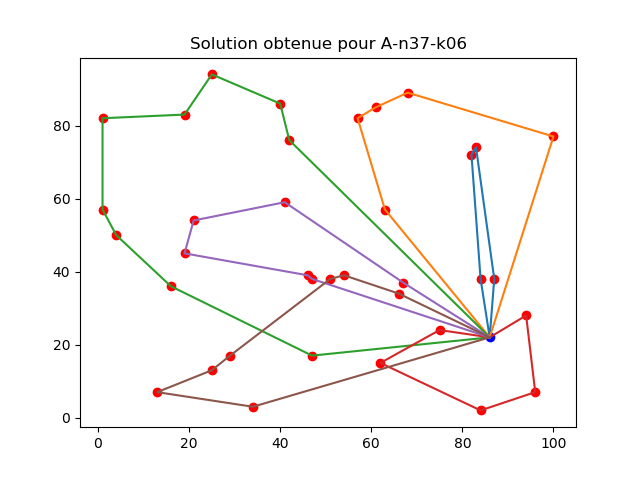
\includegraphics[scale=0.3]{solution_A-n37-k06.png}
\end{center}

\end{frame}

\begin{frame}{Comparaison}
Pour pouvoir comparer entre la solution optimale et la solution obtenue:
\begin{center}
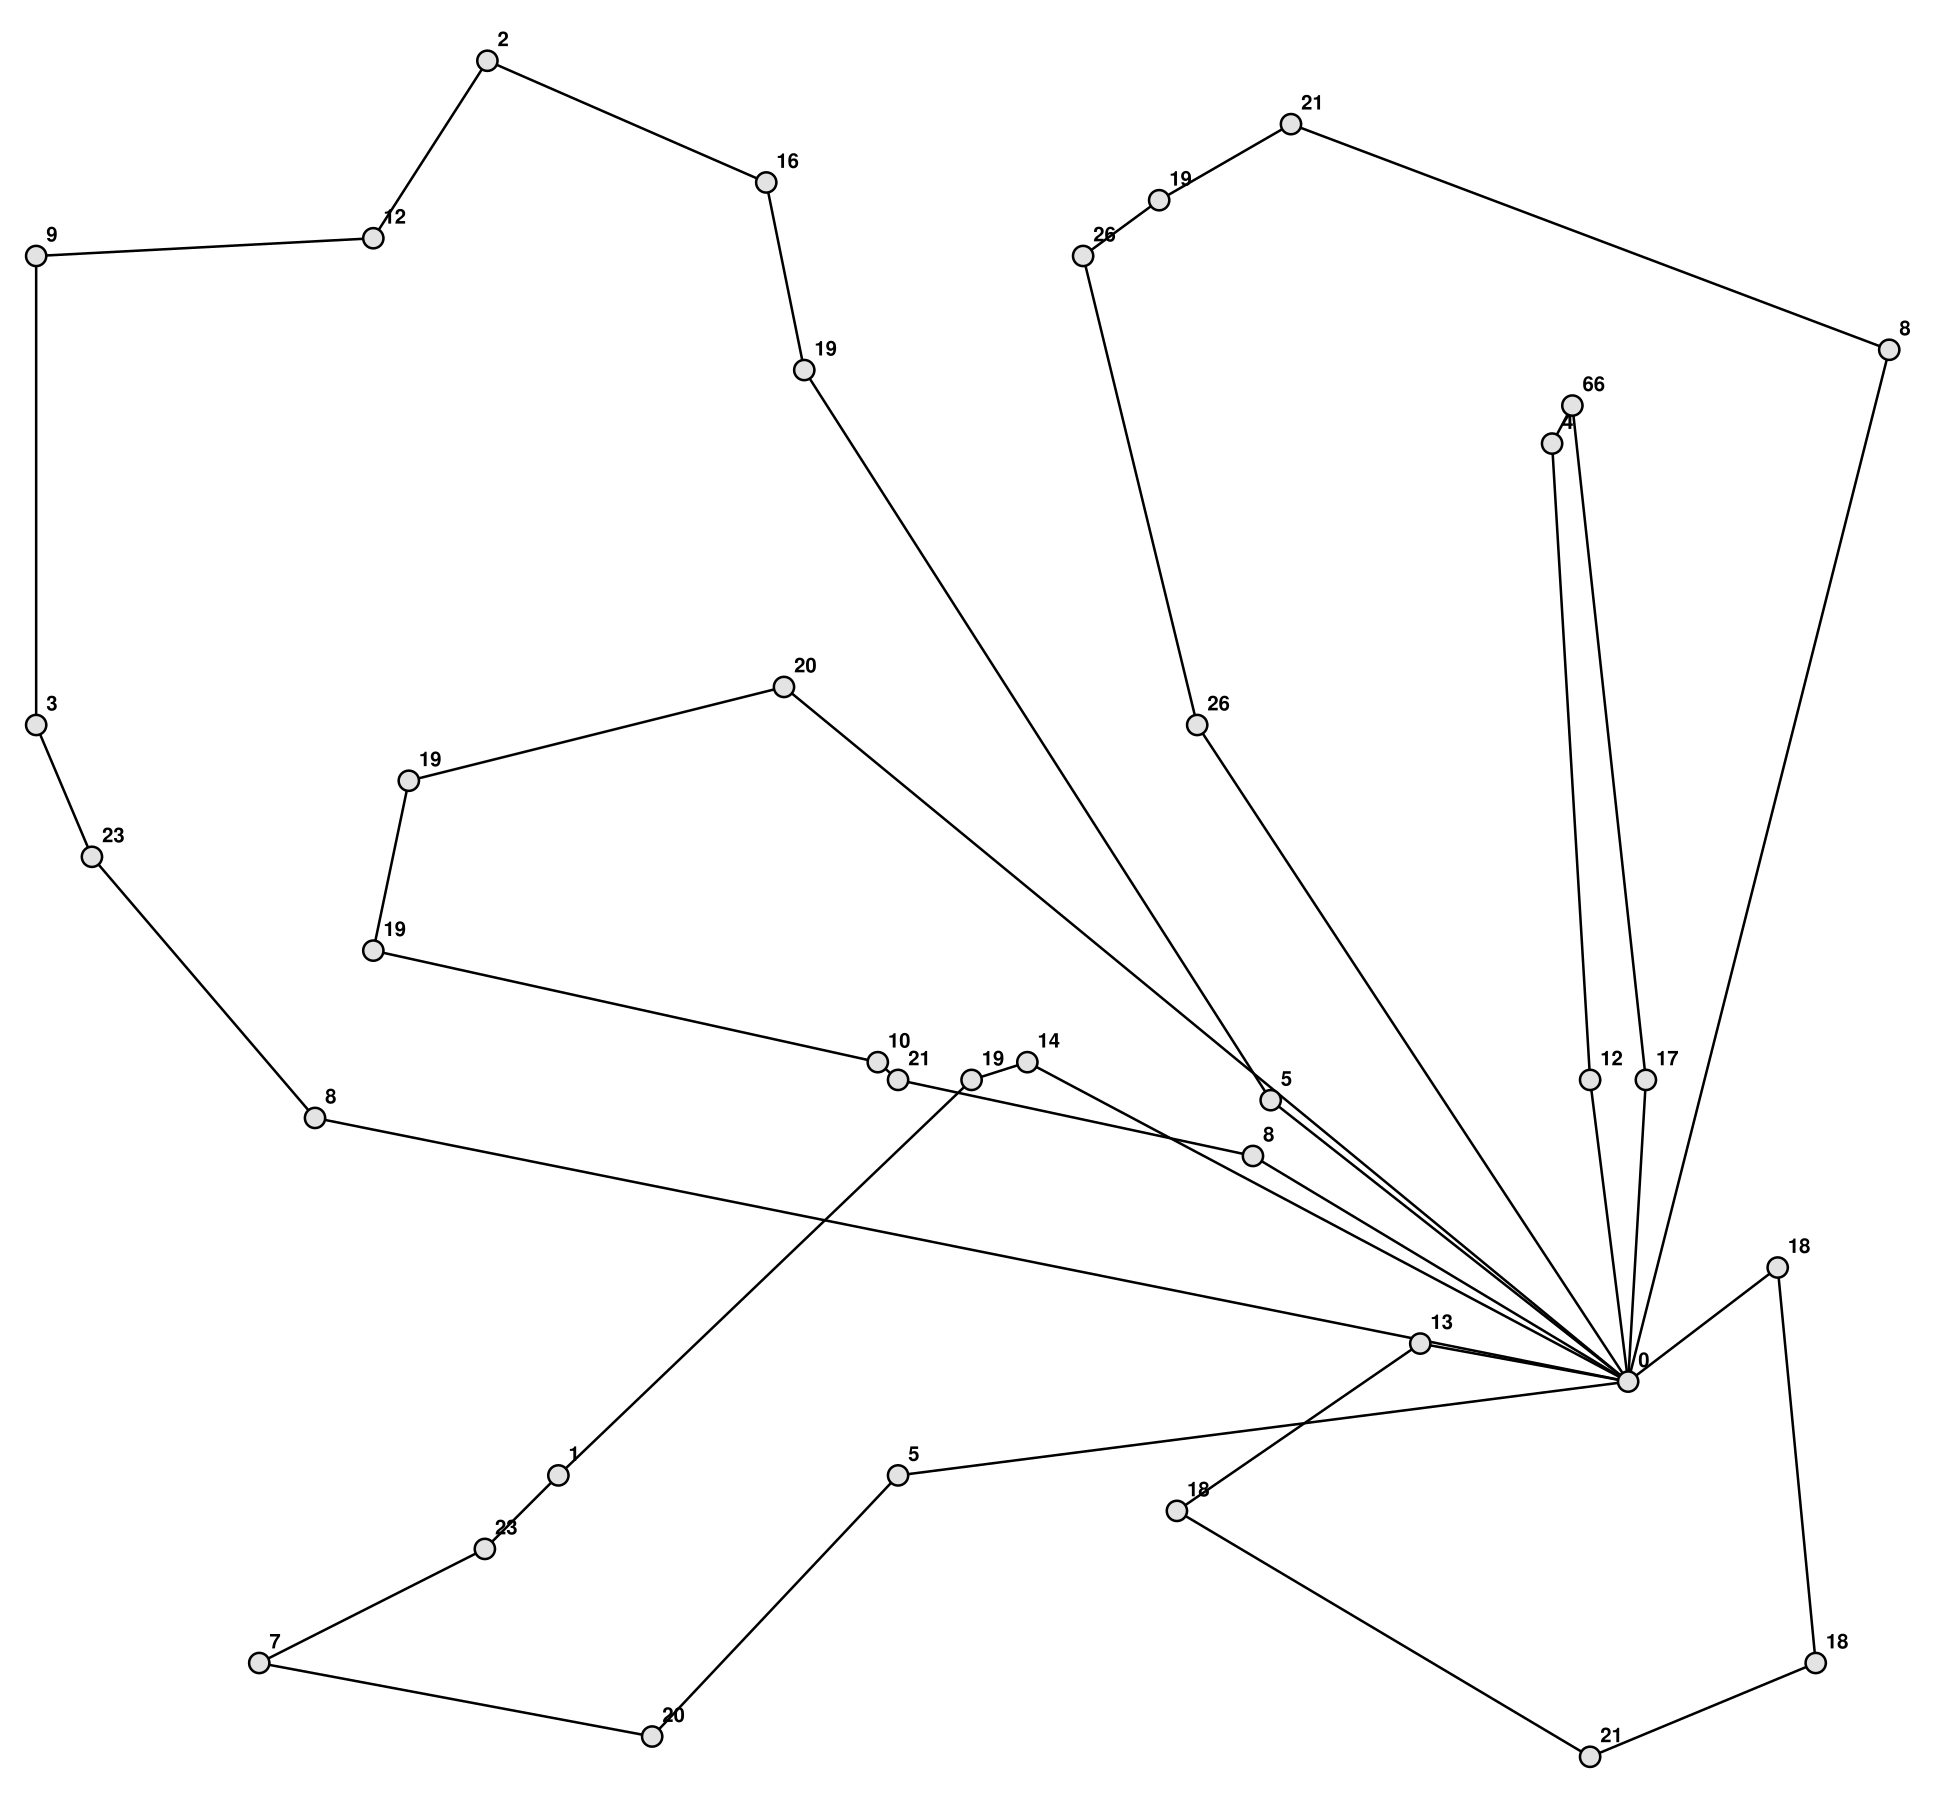
\includegraphics[scale=0.25]{A-n37-k6.png}
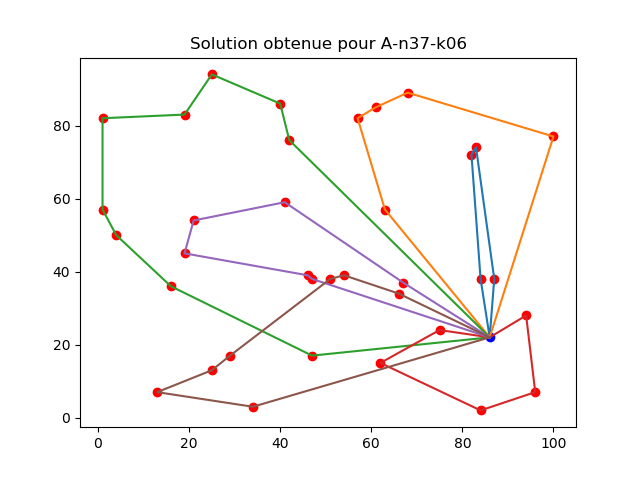
\includegraphics[scale=0.35]{solution_A-n37-k06.png}
\end{center}
Coût global de $949$ à gauche, contre $956$ à droite.
\end{frame}

\begin{frame}{Instance A-n39-k05}
Nouvelle instance choisie:
\begin{center}
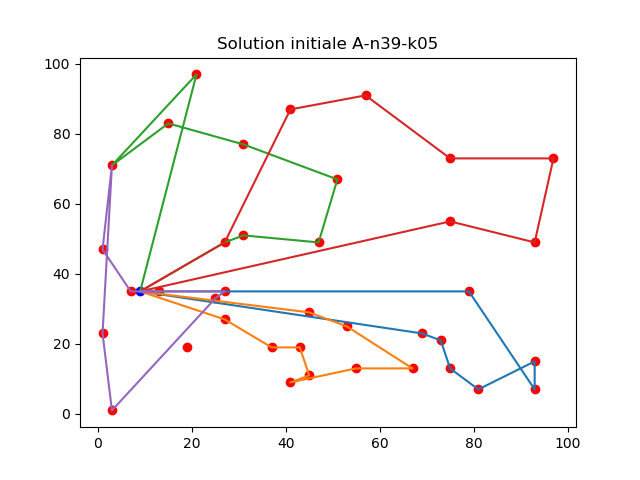
\includegraphics[scale=0.3]{initiale_A-n39-k05.png}
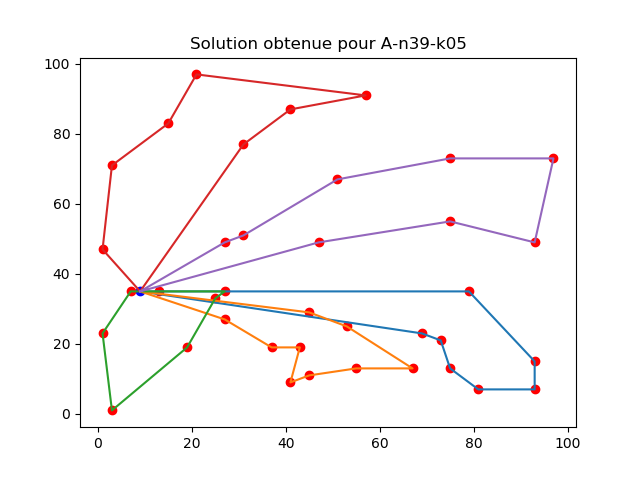
\includegraphics[scale=0.3]{solution_A-n39-k05.png}
\end{center}

\end{frame}

\begin{frame}{Comparaison}
Comparaison avec la solution optimale:
\begin{center}
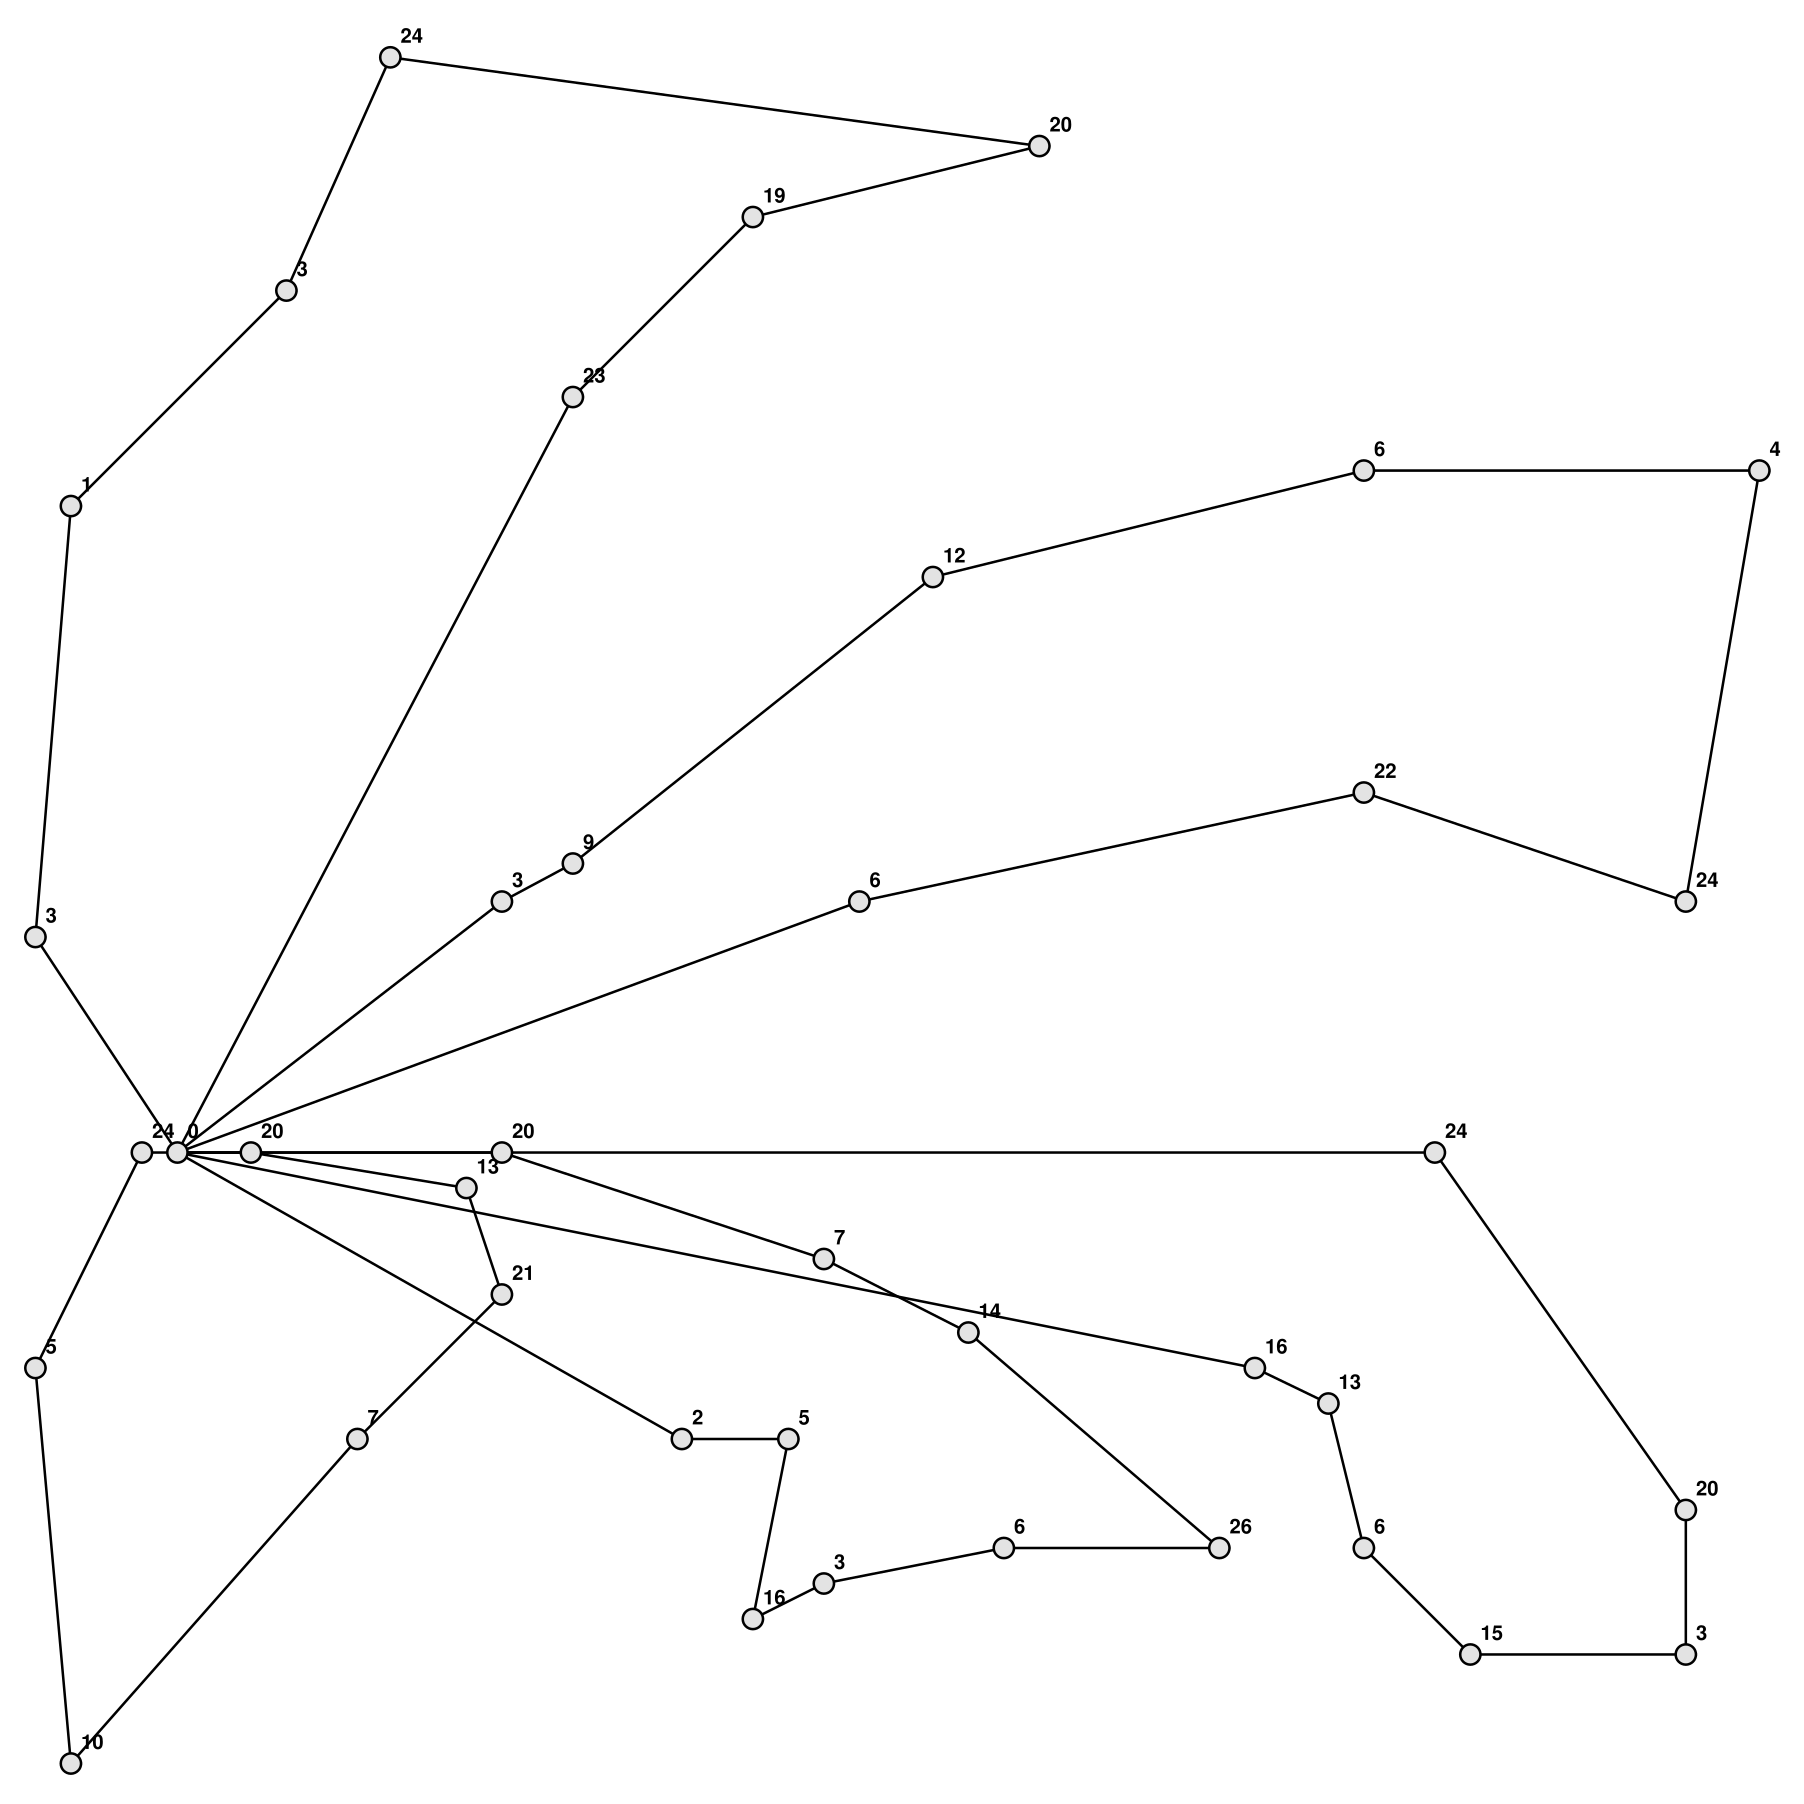
\includegraphics[scale=0.25]{A-n39-k5.png}
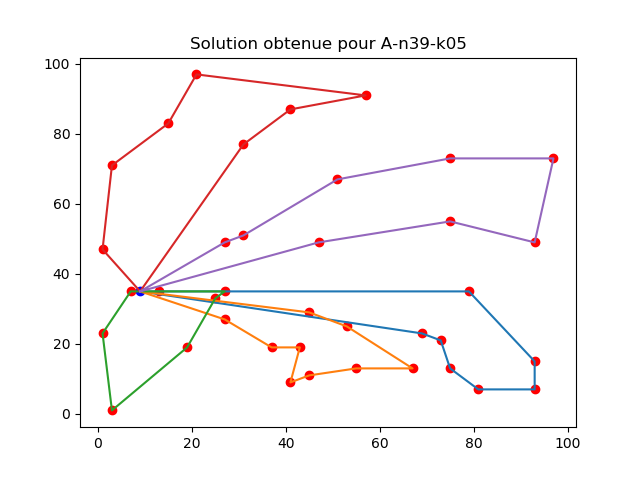
\includegraphics[scale=0.35]{solution_A-n39-k05.png}
\end{center}
Coût global de $822$ à gauche, contre $831$ à droite.
\end{frame}

\subsection{Analyse}

\begin{frame}{Paramètres utilisés}
\begin{block}
\item Calcul des 30 pp-voisins;
\item Au plus 3 déplacements dans EC;
\item $5000$ itérations.
\end{block}
\end{frame}

\begin{frame}{Pourcentage d'erreur}
a
\end{frame}

\begin{frame}{Influence solution initiale}
a
\end{frame}

\section{Arêtes communes}

\begin{frame}
a
\end{frame}

\end{document}